\sect{Base de datos}{base-datos}

El sistema gestor de base de datos utilizado para la aplicación es \monoFont{MySQL}.\ Las bases de datos de MySQL son
relacionales, lo que significa que los datos se almacenan en tablas, que están formadas por filas (campos) y columnas
(registros).\ Las tablas se relacionan entre sí mediante claves primarias y claves foráneas, que son campos que
identifican a cada registro de la tabla.
% Todo: esto es un poco básico, ¿se pone?
Este tipo de base de datos es muy empleado en aplicaciones web, por lo que es sencillo encontrar información sobre
cómo usar MySQL\@.\ Como el lenguaje de programación con el que se ha desarrollado el backend de la aplicación es
Java, se ha utilizado el ORM \monoFont{Hibernate}, que permite realizar un mapeado de la base de datos a objetos de
Java, de forma que se puede trabajar con ella de una forma transparente y cómoda para el programador.\ Para realizar
las operaciones de inserción, actualización, consulta y borrado de los datos, \monoFont{Spring Boot Data JPA} es la
mejor opción, ya que se encarga de realizar estas operaciones de forma transparente para el desarrollador,
dependiendo del nombre que reciba un método.\ También, mediante el uso de anotaciones (expresiones precedidas por el
símbolo @, como por ejemplo \monoFont{@Query}), se pueden personalizar de las consultas que se ejecutarán en base de
datos.\ El diagrama de las tablas de la base de datos de la aplicación se muestra en la siguiente figura:

\begin{figure}[H]
	\centering
	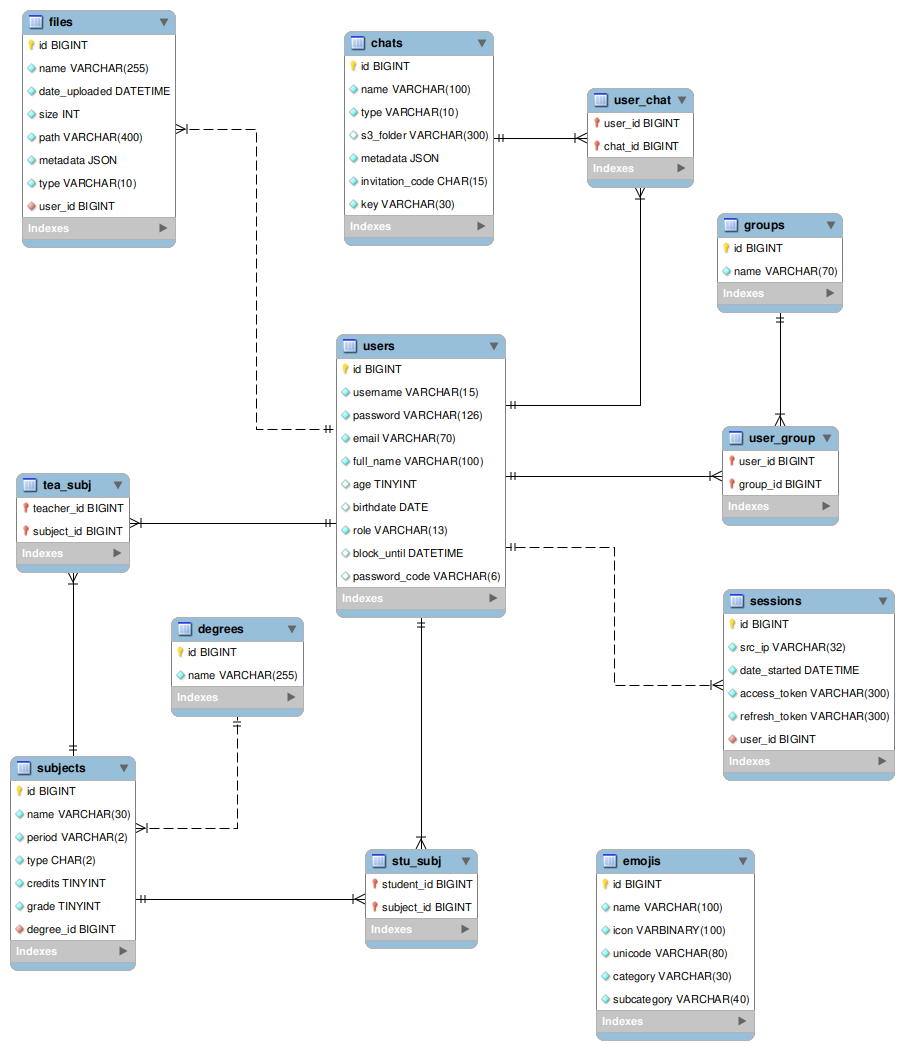
\includegraphics[width=0.8\textwidth]{diagramaBD}
	\caption{Diagrama de las tablas de la base de datos}
	\label{fig:diagrama-tablas}
\end{figure}
